\documentclass[]{krantz}
\usepackage{lmodern}
\usepackage{amssymb,amsmath}
\usepackage{ifxetex,ifluatex}
\usepackage{fixltx2e} % provides \textsubscript
\ifnum 0\ifxetex 1\fi\ifluatex 1\fi=0 % if pdftex
  \usepackage[T1]{fontenc}
  \usepackage[utf8]{inputenc}
\else % if luatex or xelatex
  \ifxetex
    \usepackage{mathspec}
  \else
    \usepackage{fontspec}
  \fi
  \defaultfontfeatures{Ligatures=TeX,Scale=MatchLowercase}
\fi
% use upquote if available, for straight quotes in verbatim environments
\IfFileExists{upquote.sty}{\usepackage{upquote}}{}
% use microtype if available
\IfFileExists{microtype.sty}{%
\usepackage[]{microtype}
\UseMicrotypeSet[protrusion]{basicmath} % disable protrusion for tt fonts
}{}
\PassOptionsToPackage{hyphens}{url} % url is loaded by hyperref
\usepackage[unicode=true]{hyperref}
\PassOptionsToPackage{usenames,dvipsnames}{color} % color is loaded by hyperref
\hypersetup{
            pdftitle={Advanced Big Data Analytics for Business with R},
            pdfauthor={Sanjeev Kumar},
            colorlinks=true,
            linkcolor=Maroon,
            citecolor=Blue,
            urlcolor=Blue,
            breaklinks=true}
\urlstyle{same}  % don't use monospace font for urls
\usepackage{natbib}
\bibliographystyle{apalike}
\usepackage{color}
\usepackage{fancyvrb}
\newcommand{\VerbBar}{|}
\newcommand{\VERB}{\Verb[commandchars=\\\{\}]}
\DefineVerbatimEnvironment{Highlighting}{Verbatim}{commandchars=\\\{\}}
% Add ',fontsize=\small' for more characters per line
\usepackage{framed}
\definecolor{shadecolor}{RGB}{248,248,248}
\newenvironment{Shaded}{\begin{snugshade}}{\end{snugshade}}
\newcommand{\KeywordTok}[1]{\textcolor[rgb]{0.27,0.27,0.27}{\textbf{#1}}}
\newcommand{\DataTypeTok}[1]{\textcolor[rgb]{0.27,0.27,0.27}{#1}}
\newcommand{\DecValTok}[1]{\textcolor[rgb]{0.06,0.06,0.06}{#1}}
\newcommand{\BaseNTok}[1]{\textcolor[rgb]{0.06,0.06,0.06}{#1}}
\newcommand{\FloatTok}[1]{\textcolor[rgb]{0.06,0.06,0.06}{#1}}
\newcommand{\ConstantTok}[1]{\textcolor[rgb]{0,0,0}{#1}}
\newcommand{\CharTok}[1]{\textcolor[rgb]{0.5,0.5,0.5}{#1}}
\newcommand{\SpecialCharTok}[1]{\textcolor[rgb]{0,0,0}{#1}}
\newcommand{\StringTok}[1]{\textcolor[rgb]{0.5,0.5,0.5}{#1}}
\newcommand{\VerbatimStringTok}[1]{\textcolor[rgb]{0.5,0.5,0.5}{#1}}
\newcommand{\SpecialStringTok}[1]{\textcolor[rgb]{0.5,0.5,0.5}{#1}}
\newcommand{\ImportTok}[1]{#1}
\newcommand{\CommentTok}[1]{\textcolor[rgb]{0.37,0.37,0.37}{\textit{#1}}}
\newcommand{\DocumentationTok}[1]{\textcolor[rgb]{0.37,0.37,0.37}{\textbf{\textit{#1}}}}
\newcommand{\AnnotationTok}[1]{\textcolor[rgb]{0.37,0.37,0.37}{\textbf{\textit{#1}}}}
\newcommand{\CommentVarTok}[1]{\textcolor[rgb]{0.37,0.37,0.37}{\textbf{\textit{#1}}}}
\newcommand{\OtherTok}[1]{\textcolor[rgb]{0.37,0.37,0.37}{#1}}
\newcommand{\FunctionTok}[1]{\textcolor[rgb]{0,0,0}{#1}}
\newcommand{\VariableTok}[1]{\textcolor[rgb]{0,0,0}{#1}}
\newcommand{\ControlFlowTok}[1]{\textcolor[rgb]{0.27,0.27,0.27}{\textbf{#1}}}
\newcommand{\OperatorTok}[1]{\textcolor[rgb]{0.43,0.43,0.43}{\textbf{#1}}}
\newcommand{\BuiltInTok}[1]{#1}
\newcommand{\ExtensionTok}[1]{#1}
\newcommand{\PreprocessorTok}[1]{\textcolor[rgb]{0.37,0.37,0.37}{\textit{#1}}}
\newcommand{\AttributeTok}[1]{\textcolor[rgb]{0.61,0.61,0.61}{#1}}
\newcommand{\RegionMarkerTok}[1]{#1}
\newcommand{\InformationTok}[1]{\textcolor[rgb]{0.37,0.37,0.37}{\textbf{\textit{#1}}}}
\newcommand{\WarningTok}[1]{\textcolor[rgb]{0.37,0.37,0.37}{\textbf{\textit{#1}}}}
\newcommand{\AlertTok}[1]{\textcolor[rgb]{0.33,0.33,0.33}{#1}}
\newcommand{\ErrorTok}[1]{\textcolor[rgb]{0.14,0.14,0.14}{\textbf{#1}}}
\newcommand{\NormalTok}[1]{#1}
\usepackage{longtable,booktabs}
% Fix footnotes in tables (requires footnote package)
\IfFileExists{footnote.sty}{\usepackage{footnote}\makesavenoteenv{long table}}{}
\usepackage{graphicx,grffile}
\makeatletter
\def\maxwidth{\ifdim\Gin@nat@width>\linewidth\linewidth\else\Gin@nat@width\fi}
\def\maxheight{\ifdim\Gin@nat@height>\textheight\textheight\else\Gin@nat@height\fi}
\makeatother
% Scale images if necessary, so that they will not overflow the page
% margins by default, and it is still possible to overwrite the defaults
% using explicit options in \includegraphics[width, height, ...]{}
\setkeys{Gin}{width=\maxwidth,height=\maxheight,keepaspectratio}
\IfFileExists{parskip.sty}{%
\usepackage{parskip}
}{% else
\setlength{\parindent}{0pt}
\setlength{\parskip}{6pt plus 2pt minus 1pt}
}
\setlength{\emergencystretch}{3em}  % prevent overfull lines
\providecommand{\tightlist}{%
  \setlength{\itemsep}{0pt}\setlength{\parskip}{0pt}}
\setcounter{secnumdepth}{5}
% Redefines (sub)paragraphs to behave more like sections
\ifx\paragraph\undefined\else
\let\oldparagraph\paragraph
\renewcommand{\paragraph}[1]{\oldparagraph{#1}\mbox{}}
\fi
\ifx\subparagraph\undefined\else
\let\oldsubparagraph\subparagraph
\renewcommand{\subparagraph}[1]{\oldsubparagraph{#1}\mbox{}}
\fi

% set default figure placement to htbp
\makeatletter
\def\fps@figure{htbp}
\makeatother

\usepackage{booktabs}
\usepackage{longtable}
\usepackage[bf,singlelinecheck=off]{caption}

\usepackage{framed,color}
\definecolor{shadecolor}{RGB}{248,248,248}

\renewcommand{\textfraction}{0.05}
\renewcommand{\topfraction}{0.8}
\renewcommand{\bottomfraction}{0.8}
\renewcommand{\floatpagefraction}{0.75}

\renewenvironment{quote}{\begin{VF}}{\end{VF}}
\let\oldhref\href
\renewcommand{\href}[2]{#2\footnote{\url{#1}}}

\makeatletter
\newenvironment{kframe}{%
\medskip{}
\setlength{\fboxsep}{.8em}
 \def\at@end@of@kframe{}%
 \ifinner\ifhmode%
  \def\at@end@of@kframe{\end{minipage}}%
  \begin{minipage}{\columnwidth}%
 \fi\fi%
 \def\FrameCommand##1{\hskip\@totalleftmargin \hskip-\fboxsep
 \colorbox{shadecolor}{##1}\hskip-\fboxsep
     % There is no \\@totalrightmargin, so:
     \hskip-\linewidth \hskip-\@totalleftmargin \hskip\columnwidth}%
 \MakeFramed {\advance\hsize-\width
   \@totalleftmargin\z@ \linewidth\hsize
   \@setminipage}}%
 {\par\unskip\endMakeFramed%
 \at@end@of@kframe}
\makeatother

\renewenvironment{Shaded}{\begin{kframe}}{\end{kframe}}

\usepackage{makeidx}
\makeindex

\urlstyle{tt}

\usepackage{amsthm}
\makeatletter
\def\thm@space@setup{%
  \thm@preskip=8pt plus 2pt minus 4pt
  \thm@postskip=\thm@preskip
}
\makeatother

\frontmatter

\title{Advanced Big Data Analytics for Business with R}
\author{Sanjeev Kumar}
\date{2018-12-16}

\let\BeginKnitrBlock\begin \let\EndKnitrBlock\end
\begin{document}
\maketitle

% you may need to leave a few empty pages before the dedication page

%\cleardoublepage\newpage\thispagestyle{empty}\null
%\cleardoublepage\newpage\thispagestyle{empty}\null
%\cleardoublepage\newpage
\thispagestyle{empty}

\begin{center}

\par\vspace*{.35\textheight}{\centering \texttt{dedicated to the one to whom I owe all} \par}

%\includegraphics{images/dedication.pdf}
\end{center}

\setlength{\abovedisplayskip}{-5pt}
\setlength{\abovedisplayshortskip}{-5pt}

{
\hypersetup{linkcolor=black}
\setcounter{tocdepth}{2}
\tableofcontents
}
\listoftables
\listoffigures
\chapter*{Preface}\label{preface}


We live in a world awash in data. Companies are increasingly turning to
data analytics to extract a competitive edge from data, especially
large, complex datasets often called \emph{Big Data}. However, companies
are increasingly facing the challenge posed by the scarcity of
analytical talent - people who can turn data into better decisions,
people who can extract insights and information from data. There is
growing demand for professionals with strong quantitative skills
combined with an understanding of how data analytic techniques can be
applied to business contexts and managerial decision making. To help my
students succeed in this growing field, I teach classes in
\textbf{Advanced Big Data Analytics} in Ross School of Business, Univ.
of Michigan. In these courses I teache advanced analytical, statistical
and data mining tools with an applied focus. This book is developed
specifically for these courses.

The main focus of this book (and the associated coures) is to prepare
students to model and manage business decisions with data analytics and
decision models using real life case contexts and datasets. By the end
of this book students will have a better understanding of processes,
methodologies and tools used to transform the large amount of business
data available into useful information and support business decision
making. The book will focus on extracting actionable business
intelligence by analyzing traditional business data as well as more
recently available datasets such as social media, crowdsourcing and
recommendation engines. The book focuses on the powerful, open source
(and hence free) data analysis environment R.

As I designed these courses, I realized that while there are a lot of
references available for doing Advanced Analytics on Big Data using R,
there isn't a good reference that approaches the topic from the
perspective of business students and is accessible for students who do
not have extensive background in statistics or computer programming. I
designed my classes to have an applied nature with significant amount of
hands-on work on real business Big Data with significant managerial
implications. I emphasized aspects of the analytics process that are
important for actual practice of data science but are not typically well
covered in traditonal textbooks - like data cleaning, managing large
datasets and building data dashboards. I ended up creating a significant
amount of material for the classes - much of it collated from already
available but widely dispersed sources. This book is a collection of
these material.

Business students have a unique mixture of tech savvy, super smarts and
learning ability with a relative lack of computer programming or coding
experience. They further have a great applied sense of statistics and
data analysis but typically without the theoretical expertise of a
Statistics student. This book is directed towards such students. This
book assumes that business students are joining an Advanced Analytics
course without any knowledge of computer programming and without any
background in R. This book assumes that students are familiar with basic
probability and statistics but their focus is on applied statistics -
not on the theory. The book then builds up student's comfort level with
R while at the same time makeing progress on key Advanced Analytics
materials.

Direct all feedback on this book to the author at
email:\texttt{sankum\ at\ umich.edu} or twitter: \texttt{@a\_teachr}

\section*{Structure of the book}\label{structure-of-the-book}


Add structure information for the book here.

\section*{Software information and
conventions}\label{software-information-and-conventions}


This book is built using the \textbf{knitr}\index{knitr} package
\citep{xie2015} and the \textbf{bookdown}\index{bookdown} package
\citep{R-bookdown}. Following is the R session information that built
the current version:

\begin{Shaded}
\begin{Highlighting}[]
\NormalTok{xfun}\OperatorTok{::}\KeywordTok{session_info}\NormalTok{()}
\end{Highlighting}
\end{Shaded}

\begin{verbatim}
## R version 3.5.1 (2018-07-02)
## Platform: x86_64-w64-mingw32/x64 (64-bit)
## Running under: Windows 7 x64 (build 7601) Service Pack 1
## 
## Locale:
##   LC_COLLATE=English_United States.1252 
##   LC_CTYPE=English_United States.1252   
##   LC_MONETARY=English_United States.1252
##   LC_NUMERIC=C                          
##   LC_TIME=English_United States.1252    
## 
## Package version:
##   backports_1.1.2 base64enc_0.1.3 bookdown_0.8   
##   compiler_3.5.1  digest_0.6.16   evaluate_0.11  
##   glue_1.3.0      graphics_3.5.1  grDevices_3.5.1
##   highr_0.7       htmltools_0.3.6 jsonlite_1.5   
##   knitr_1.20      magrittr_1.5    markdown_0.8   
##   methods_3.5.1   mime_0.5        Rcpp_0.12.18   
##   rmarkdown_1.10  rprojroot_1.3-2 stats_3.5.1    
##   stringi_1.1.7   stringr_1.3.1   tinytex_0.8    
##   tools_3.5.1     utils_3.5.1     xfun_0.3       
##   yaml_2.2.0
\end{verbatim}

Package names are in bold text (e.g., \textbf{rmarkdown}), and inline
code and filenames are formatted in a typewriter font (e.g.,
\texttt{knitr::knit(\textquotesingle{}foo.Rmd\textquotesingle{})}).
Function names are followed by parentheses (e.g.,
\texttt{bookdown::render\_book()}).

\section*{Acknowledgments}\label{acknowledgments}


Add acknowledgements here.

\BeginKnitrBlock{flushright}
Sanjeev Kumar\\
Technology and Operations, Ross School of Business, Univ. of Michigan
\EndKnitrBlock{flushright}

\chapter*{About the Author}\label{about-the-author}


Sanjeev Kumar is part of the Technology and Operations faculty at the
Ross School of Business, Univ. of Michigan, Ann Arbor.

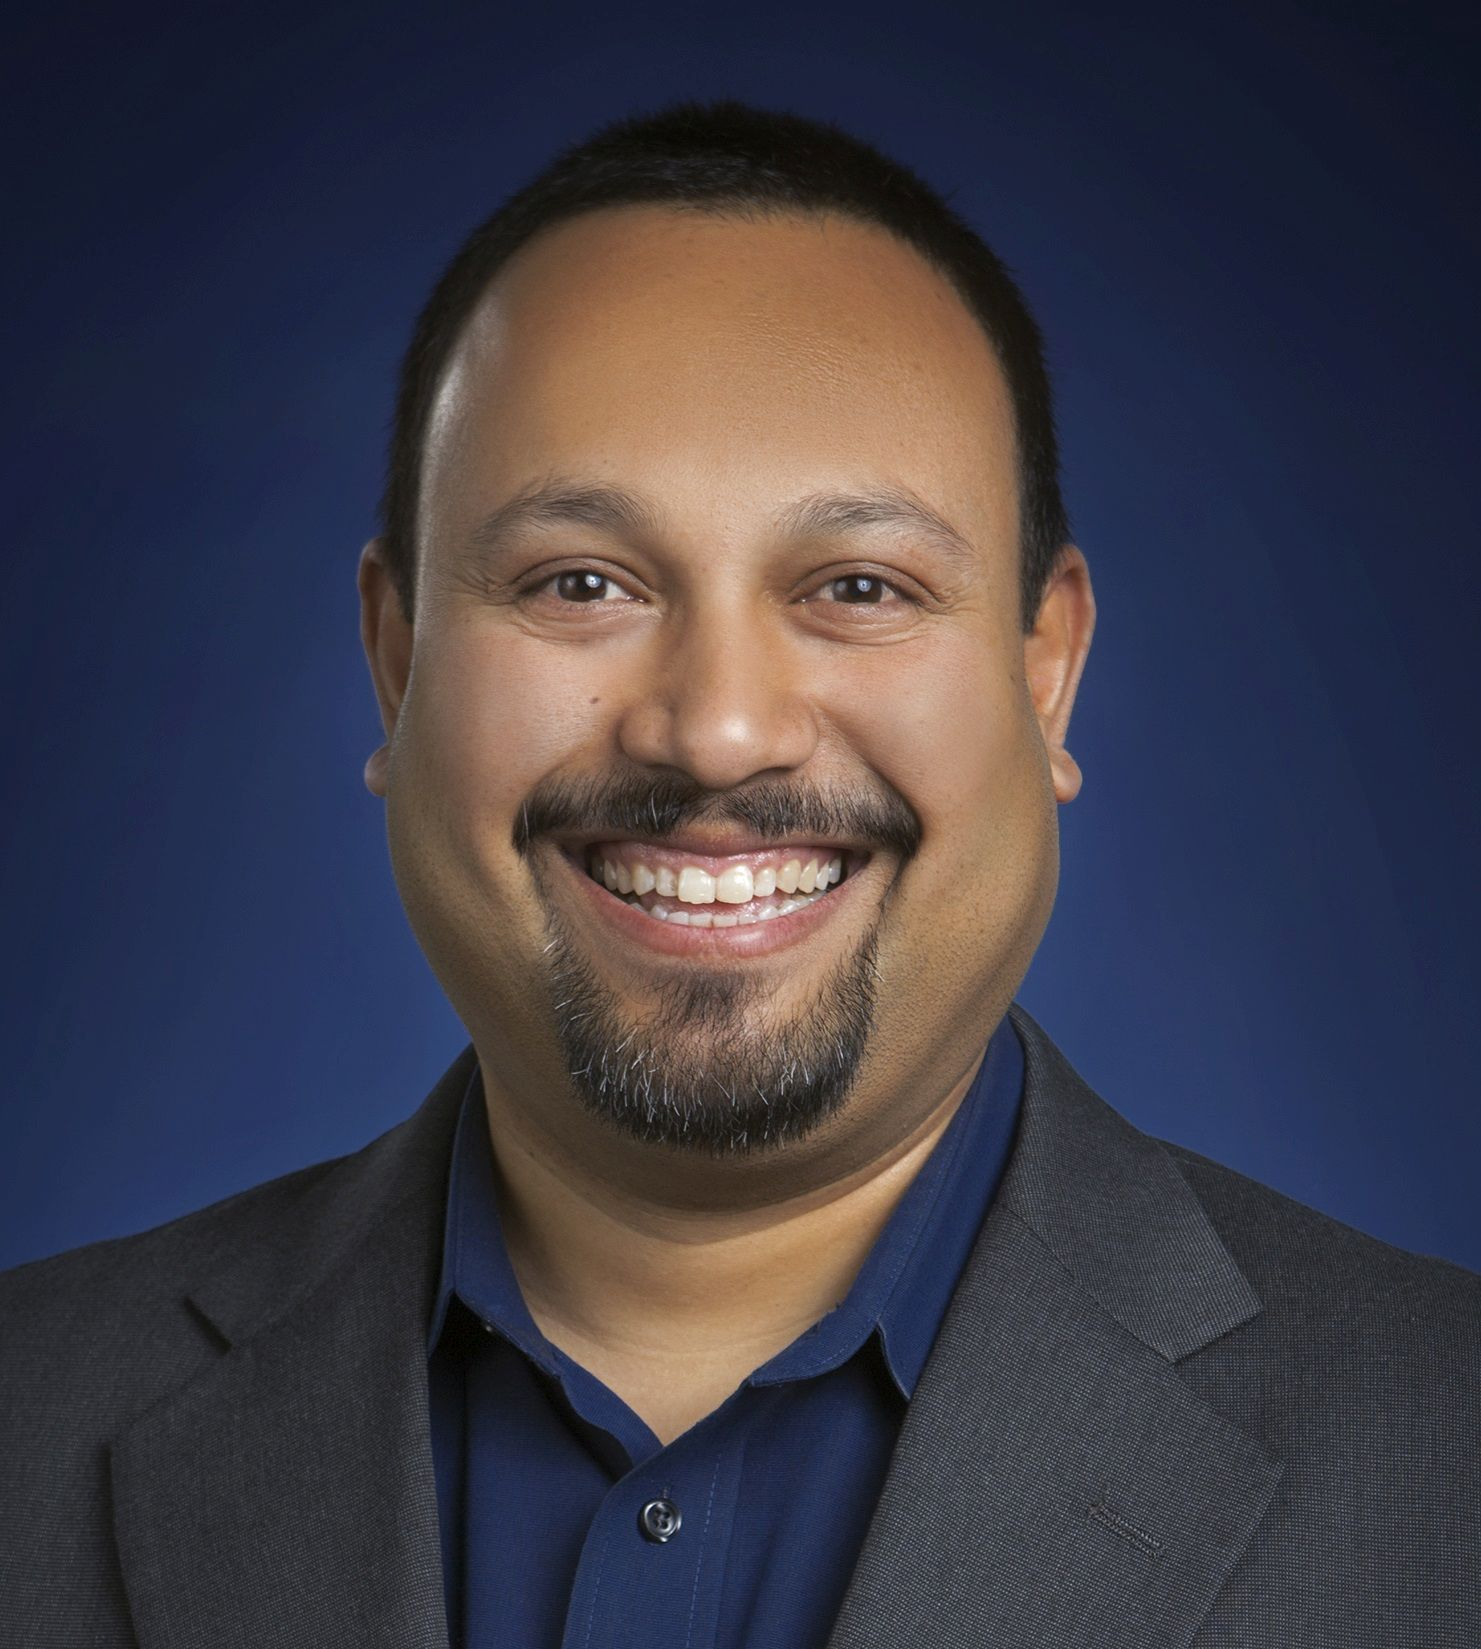
\includegraphics{images/SanjeevKumar.jpg} \{-\}

\mainmatter

\chapter{Introduction}\label{introduction}

Welcome to \textbf{Advanced Big Data Analytics for Business with R}.
Let's get started.

\section{Who Is This Book For?}\label{who-is-this-book-for}

This book is for business students, practitioners and executives who
want to have hands-on experience in working with business related big
data and want to extract actionable insights from the data using
advanced analytical techniques. This book is application oriented and
hence focuses on the application of advanced analytical techniques
rather than the theoretical details. Consequently, this book is not for
readers solely focused on the theoretical, statistical part of data
analytics.

This book assumes that the readers have basic familiarity with
introductory probability and statistics. This domain is easier to follow
and understand if the reader also has \emph{some} exposure to
\emph{some} kind of computer programming although that is not a
necessity. This book has been written for a practitioner audience, not
an academic one. The book aims to be an exhaustive reference resource
for practitioners - that's why it starts with baby steps of introducing
R and basic data manipulation and ends at the other end with advanced
Machine Learning algorithms and complex model improvement algorithms.

Thank you for placing your trust in this book. This chapter will
provider further details about this book and how to best read/use this
book.

\section{About This Document}\label{about-this-document}

This document, which you are probably seeing as a GitHub eBook or a PDF
document or even as printed book, has been written entirely using R and
RStudio. It uses the R packages \texttt{bookdown} along with
\texttt{rmarkdown} to integrated R code inside my favorite document
creation system called \textbf{LaTeX}. This document has been created
entirely using Open Source tools and has been released back into the
Open Source ecosystem for free using the GNU General Public License
(GPL). You are free to share this document with others as long as you
comply with the GPL license. GPL License usually require that the
product (in this case, this book) be made available free or charge; and
any subsequent product made using the GPL Licensed product must also be
made available free of charge \citep{TheGNUGe51:online}.

This is my first attempt at writing a book size document. I have had to
develop a bunch of workarounds to make the process work and get a
quality output. The source code for this book is available for public
use free of charge at: \url{https://github.com/clarifyR/AABookDown}.

\section{How is This Book Structured}\label{how-is-this-book-structured}

This book covers a wide range of material. The material is organized in
5 parts, 19 chapters and several appendices.

\subsection{Part I: Getting Started}\label{part-i-getting-started}

We set ourselves for the book - download and install all needed
software; figure our way around R and RStudio and learn the basics of
the R language. Essentially lay down enough of a foundation that we can
start getting productive. For students without a computer programming
background, it is essential that they do not rush this part. Our success
in later parts depend upon us getting comfortable with the material
here.

\subsection{Part II: Data Exploration and
Visualization}\label{part-ii-data-exploration-and-visualization}

Real data analytics begins with us understanding and getting a handle on
the data. This typically involves cleaning up the data, generating
descriptive statistics to better understand the data and finally
creating visualizations that allow us to better understand the
underlying complexity of the data. In my opinion, data cleaning is the
most under-appreciated part of data analytics. It often takes more time
and effort than the actual analysis that follows.

Data visualization has emerged as a key tool in Big Data Analytics. We
specifically focus our attention here on a subset of data visualization
that is important in the business context - creating data dashboards
that can help managerial decision making.

\subsection{Part III: Traditional Statistical
Modeling}\label{part-iii-traditional-statistical-modeling}

Even advanced analytic techniques like machine learning algorithms in
the next part have their foundations in traditional statistical
methodologies. Classical statistical modeling approaches like Linear
Regression are still the benchmark given their immense popularity,
flexibility and stability. In this part of the book, we explore
traditional statistical analysis tools like Linear Regression,
Generalized Linear Models like Logistic and Survival Models, Principal
Components and Factor Analysis, Time Series Analysis and so on.

As we assume that you are already familiar with basic probability and
statistics, we will focus on application of the methodologies and not
the underlying theory. We will also focus on how to tweak these tools
for the Big Data world as many of these tools run into trouble when
sample sizes are quite large. Bigger is not always better - traditional
statisticall methodologies were developed/optimized for smaller sample
sizes. Using them for large sample sizes give rise to unique issues and
problems - we will discuss how to address them.

\subsection{Part IV: Machine Learning and Predictive
Analytics}\label{part-iv-machine-learning-and-predictive-analytics}

This is the largest and the most important part of the book. This is why
this book was written in the first place - an overview of data analytics
tools specific to Big Data - variously known as Machine Learning,
Statistical Learning, Predictive Analytics, Data Mining as so on. This
book focuses on tools that help us make sense of Big Data and helps us
automate the extraction of managerial decision making insights from Big
Data.

As with much of the rest of the book, the focus is on applying the tools
rather than their theoretical/mathematical underpinnings. We will
discuss enough theory to develop an overall understanding and then
devote our energies on making these tools work on real datasets.

\subsection{Part V: Putting It All
Together}\label{part-v-putting-it-all-together}

Now that we have gone through all the elements individually, we can move
forward to create a combined, integrated approach that puts all these
pieces together. How to combine different models so that they result in
an output better than sum of their parts? How to ensure that our models
improve as more data become available?

We will conclude by running a couple of large integrated data analytics
projects that will combine elements discussed in the book.

\subsection{Part V: Appendices, Bibliography and
Index}\label{part-v-appendices-bibliography-and-index}

Back matter of the book. The Index in the end has three main components
- Key Concepts, R Commands and R Packages. Appendices include syllabus
for the two courses this book is primarily used for and other
miscellaneous content that did not fit in one of the main matter
chapters.

There are a lot of quality, free, online resources available for
building up your R and Data Analytics skills before you go through this
book or the associated courses. They are listed in Appendix: Key
References. A fully fleshed data analysis example has been presented on
Appendix: Data Analysis Example to give you an idea of the power and
range of what can be accomplished with just a little bit of familiarity
with R.

\section{How to Read This Book}\label{how-to-read-this-book}

You would have noticed by now that this book integrates R code within
its text. Most of the time R code takes the form of dedicated code
blocks like the one below:

\begin{Shaded}
\begin{Highlighting}[]
\CommentTok{#This is a demo code block}
\KeywordTok{print}\NormalTok{(}\StringTok{"Hello World"}\NormalTok{)}
\end{Highlighting}
\end{Shaded}

\begin{verbatim}
## [1] "Hello World"
\end{verbatim}

As you can see from above, code blocks are printed in color, in
\texttt{fixed\ width\ font}. There is a color scheme here that you will
soon become familiar with - comments are in italics and kind of violet
looking, functions are in reddish color, strings appear bluish and so
on. The output of the code block appears right after - for example - the
output of the \texttt{print()} command follows the code above.

You would notice that whenever we refer to a R command in a significant
way (like \texttt{print()} in paragraph above), the command is printed
in \texttt{fixed\ width\ font}, in red color with a yellow highlight
that makes it easy for you to see which commands are discussed
significantly on the page. The highlighting also ensures that an entry
for the command is placed in the Index provided at the end of the book.
For times when a command is mentioned in text in a minor way not
necessating a margin and Index entry, they will be typed in
\texttt{fixed\ width\ font}.

Like R Commands, this book provides special formatting for R Packages
used in the book. R Packages are fomatted like R Commands but in blue
color - check our reference of the \texttt{clarifyR} package earlier -
blue fixed width font text with yellow highlighting and finally an entry
in the Packages section of the Index.

Lastly, special formatting is provided for key concepts - similar to R
Commands and Packages in all respects except that they are in bolded and
in black color and their Index entry is in the Key Concepts section. For
example: this book focuses on \texttt{Open\ Source} software - that are
created by a community of software developers for use by the community,
usually made available for free.

The three special formatting elements - commands, packages and key
concepts - ensure that you have a summary of significant elements
discussed in the page just by looking for highlighted items.

\section*{Is This Book Suitable For You?}

Well - you wouldn't know until you spend some time with it. Dig in.

A quick word of caution though before you get too deep: this book (and
the associated courses) are very hands-on. There is no point in reading
this book like a sequence of text. This book should be seen more as an
illustrated text - illustrated with relevant R commands and material.
You should read this book alongside an RStudio session - trying all the
commands there as you read along. You will need to get comfortable with
a lot of command line typing, keyboard shortcuts and figuring
workarounds to inevitable problems that will arise. We will often get
into situations where there will be no tested/optimized/prescribed
solution and we will need to figure our way out - often with some trial
and error. You should be comfortable with such ambiguity.

\section{Archive - Delete}\label{archive---delete}

This section holds the placeholder information that will be deleted
after the book is built.

We have a nice figure in Figure \ref{fig:hello}, and also a table in
Table \ref{tab:iris}.

\begin{Shaded}
\begin{Highlighting}[]
\KeywordTok{par}\NormalTok{(}\DataTypeTok{mar =} \KeywordTok{c}\NormalTok{(}\DecValTok{4}\NormalTok{, }\DecValTok{4}\NormalTok{, }\DecValTok{1}\NormalTok{, .}\DecValTok{1}\NormalTok{))}
\KeywordTok{plot}\NormalTok{(cars, }\DataTypeTok{pch =} \DecValTok{19}\NormalTok{)}
\end{Highlighting}
\end{Shaded}

\begin{figure}
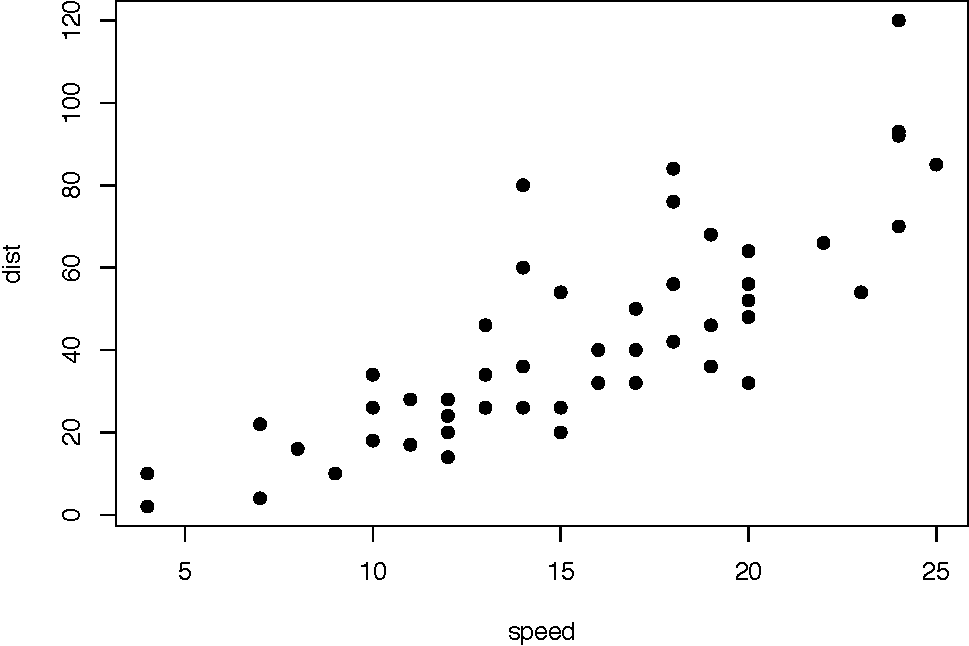
\includegraphics[width=0.9\linewidth]{bookdown_files/figure-latex/hello-1} \caption{Hello World!}\label{fig:hello}
\end{figure}

\begin{Shaded}
\begin{Highlighting}[]
\NormalTok{knitr}\OperatorTok{::}\KeywordTok{kable}\NormalTok{(}
  \KeywordTok{head}\NormalTok{(iris), }\DataTypeTok{caption =} \StringTok{'The boring iris data.'}\NormalTok{,}
  \DataTypeTok{booktabs =} \OtherTok{TRUE}
\NormalTok{)}
\end{Highlighting}
\end{Shaded}

\begin{table}

\caption{\label{tab:iris}The boring iris data.}
\centering
\begin{tabular}[t]{rrrrl}
\toprule
Sepal.Length & Sepal.Width & Petal.Length & Petal.Width & Species\\
\midrule
5.1 & 3.5 & 1.4 & 0.2 & setosa\\
4.9 & 3.0 & 1.4 & 0.2 & setosa\\
4.7 & 3.2 & 1.3 & 0.2 & setosa\\
4.6 & 3.1 & 1.5 & 0.2 & setosa\\
5.0 & 3.6 & 1.4 & 0.2 & setosa\\
5.4 & 3.9 & 1.7 & 0.4 & setosa\\
\bottomrule
\end{tabular}
\end{table}

\chapter{Advanced Big Data Analytics}\label{advanced-big-data-analytics}

We talk about the \emph{FOO} method\index{FOO} in this chapter.

\cleardoublepage 

\appendix \addcontentsline{toc}{chapter}{\appendixname}


\chapter{Syllabi}\label{syllabi}

This appendix will have the syllabus for the relevant Ross courses.

\section{TO404 Big Data Manipulation and
Visualization}\label{to404-big-data-manipulation-and-visualization}

\section{TO414 Advanced Analytics}\label{to414-advanced-analytics}

\section{TO628 Advanced Big Data
Analytics}\label{to628-advanced-big-data-analytics}

\bibliography{book.bib,packages.bib}

\backmatter
\printindex

\end{document}
